\documentclass[12pt]{ctexart}

\title{机械设计基础课程设计报告}
\author{欧 宇恒}
\date{\today}
\usepackage{ctex}			%处理中文字体宏包
\usepackage{graphicx}		%处理图片宏包
\usepackage{amsmath}		%处理数学公式宏包	
\usepackage{setspace}		%处理行距宏包
\usepackage[left=1.91cm,right=1.91cm,top=2.54cm,bottom=2.54cm]{geometry}		%编辑页面格式
\usepackage{booktabs}		%处理三线表宏包
\usepackage{color}			%处理颜色宏包
\usepackage{multirow}       %处理合并单元格宏包


\begin{document}	
	\ctexset{
		section={
			name={\S},
			nameformat={\zihao{2}},
			titleformat={\centering\heiti\zihao{2}},
		},
		subsection={
			name={},
			nameformat={\zihao{4}},
			titleformat={\zihao{4}},
		},
	}

    
\begin{titlepage}

    \begin{center}
    % Upper part of the page
    
\includegraphics[width=0.4\textwidth]{./CSU.png}\\[1cm]    
    \textsc{\LARGE Central South University}\\[1.5cm]
    \textsc{\Large Final Week Project}\\[1.5cm]
    % Title
    \textsc{\huge \bfseries 机械设计基础课程设计说明书}\\[1.5cm]
    % Author and supervisor
    \begin{minipage}{0.4\textwidth}
    \begin{flushleft} \large
    \emph{Author:}\\
    OuYuheng
    \end{flushleft}
    \end{minipage}
    \begin{minipage}{0.4\textwidth}
    \begin{flushright} \large
    \emph{Supervisor:} \\
    Dr.Zhou \textsc{Ying}
    \end{flushright}
    \end{minipage}
    
    \vfill
    
    % Bottom of the page
    {\large \today}
    
    \end{center}
    
    \end{titlepage}
%%封面


%%封面 end

\newpage

\tableofcontents

\newpage

\section{运动参数、动力参数的确定}

\subsection{电动机型号选择}

根据所给题目要求,本小组已知参数为输送带的牵引力$F=3.5\text{kN}$,输送带的速度$v=1.8\text{m/s}$,输送带滚筒直径$D=350\text{mm}$,由此可以计算出工作机所需功率 (kW):

$$P_W=Fv=33.5\times 1.8=6.3\text{kW}$$

其次,通过查表 [2]P7 表 2-4,可得齿轮、轴承、联轴器的传动效率,依据本题具体情况,取各传动效率如下:

\begin{table}[h]
    \centering
    \begin{tabular}{c c}
        \toprule
        传动构建 & 效率 \\
        \midrule
        V 带 & 0.96\\
        滚动轴承 & 0.98\\
        齿轮 & 0.96\\
        联轴器 & 0.99\\
        \bottomrule
    \end{tabular}
    \caption{各传动构件传动效率}
\end{table}

故可得总传动效率为:

$$\eta_\text{总} = \eta_\text{带}\eta^3_{\text{轴承}}\eta_{\text{齿轮}}\eta_{\text{联轴器}}=0.96\times 0.98^3\times 0.96\times 0.99 = 0.86$$

由此可以计算出电动机需要提供的输入功率:

$$P_d = \frac{P_W}{\eta_\text{总}} = \frac{6.3}{0.86} = 7.33\text{kW}$$

本小组选取电动机转速为 $1000\text{r/min}$,考虑到选择的电动机功率$P_d'>P_d$,故通过查阅 [2]P196 表 20-1 得到应选取电动机型号为 Y160M-6,该型号电动机的额定满载转速为$n_m=970\text{r/min}$。

对于输出卷筒而言,计算其工作转速为:

$$n_W = \frac{60000v}{\pi D} = \frac{60000\times 1.8}{\pi \times 350} = 98\text{r/min}$$

故可得减速器的总传动比为:

$$i_\text{总} = \frac{n_m}{n_W}=\frac{970}{98}=9.87$$

本课设中,选取齿轮传动比为 3.06,则此时带传动比为 3.23,均在要求范围之内。选取小齿轮齿数为 29,大齿轮齿数为 89,满足齿轮传动比要求,并且齿数互质,有较好的传动性能。

\subsection{运动参数与动力参数计算}

\begin{figure}[htbp]
    \centering
    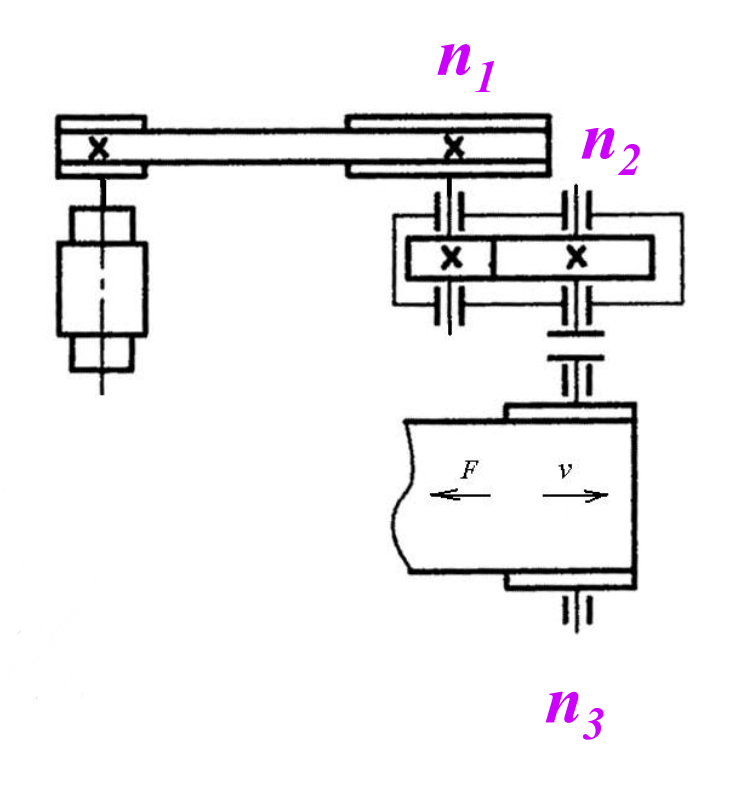
\includegraphics[scale=0.2]{dynamic_argument.png}
    \quad
    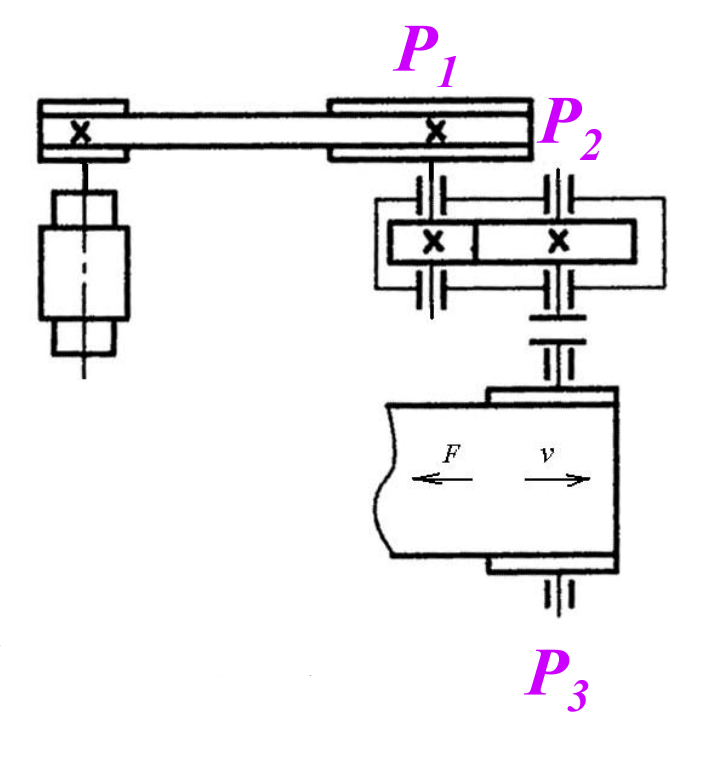
\includegraphics[scale=0.2]{P.png}
    \caption{各机构运动转速与工作功率示意图}\label{figure1}
\end{figure}

各构件工作转速和工作功率如图\ref{figure1}所示,通过传动比计算可得:

$$n_1=\frac{n_m}{i_\text{带}}=\frac{970}{3.23}=301\text{r/min}$$

$$n_2=\frac{n_1}{i_{\text{齿轮}}}=n_3=n_W=98\text{r/min}$$

各个轴的功率计算:

$$P_1 = P_d\eta_{\text{带}}=7.5\times 0.96 = 7.2$$

$$P_2 = P_1 \eta_{\text{轴承}}\eta_{\text{齿轮}}=7.2\times 0.98\times 0.96 = 6.77$$

$$P_3 = P_2 \eta_{\text{轴承}}\eta_{\text{联轴器}}=6.77\times 0.98\times 0.99$$

各轴上都是以该轴上的最大功率(即:输入功率)作为设计所用,故可以算出各轴上的传动力矩:

$$T_1 = 9550\frac{P_1}{n_1} = 9550\times \frac{7.2}{301}=228.66\text{kN·m}$$

$$T_2 = 9550\frac{P_2}{n_2} = 9550\times \frac{6.77}{98}=658.27\text{kN·m}$$

$$T_3 = 9550\frac{P_3}{n_3} = 9550\times \frac{6.57}{98}=645.10\text{kN·m}$$

将以上结果汇总后,得到表\ref{table1},列出了各个轴的输入功率、工作转速与传动扭矩,至此,课程设计的运动参数和动力参数确定完毕。

\begin{table}[h]
    \centering
    \begin{tabular}{c c c c c}
        \toprule
        轴号 & 功率$P/\text{kW}$ & 转速$N/\text{(r/min)}$ & 扭矩$T/\text{kN·m}$ & 传动比$i$ \\
        \midrule
        电机轴 & 7.5 & 970 & 73.84 & \multirow{ 2}{*}{$i_{\text{带}}=3.23$}\\
        I & 7.2 & 301 & 228.7 & \\
        II & 6.77 & 98 & 658.27 & \multirow{ 2}{*}{$i_{\text{齿轮}}=3.06$}\\
        III & 6.57 & 98 & 645.10 & \\
        \bottomrule
    \end{tabular}
    \caption{运动参数与动力参数汇总表}\label{table1}
\end{table}
    


\section{齿轮设计计算方法}

本课程设计选用闭式齿轮进行齿轮设计,
设齿轮传动比$i_{12}=3.1$,
高速轴转速$n_1=301 \text{r/min}$,
传动功率$P=7\text{kW}$,
考虑到该课程设计中的齿轮需有较好的接触疲劳强度,
故采用软齿面设计,
通过参考文献 [1]P179 提供的方法对齿轮进行设计。

\subsection{选择材料及确定许用应力}

小齿轮采用 45 号调质钢作为材料,
并作调质热处理,
齿面硬度为 $197\sim 286\text{HBS}$,
接触疲劳极限为$\sigma_{Hlim}=550\sim 620\text{MPa}$,
弯曲疲劳极限$\sigma_{FE}=410\sim 480\text{MPa}$,
此时相应的疲劳强度取均值得,
$\sigma_{Hlim1} = 585\text{MPa}$,
$\sigma_{FE1}=445\text{MPa}$,
由于大小齿轮均为软齿面,考虑到小齿轮齿根较薄时,弯曲强度较低,受载次数多,故对大齿轮做正火热处理,使得小齿轮的弯曲疲劳极限稍高于大齿轮,大、小齿轮的弯曲强度近乎相近

故此时对大齿轮而言,
齿面硬度为 $156\sim 217\text{HBS}$,
接触疲劳极限为$\sigma_{Hlim}=350\sim 400\text{MPa}$,
弯曲疲劳极限$\sigma_{FE}=280\sim 340\text{MPa}$,
此时相应的疲劳强度取均值得,
$\sigma_{Hlim2} = 375\text{MPa}$,
$\sigma_{FE2}= 310\text{MPa}$
(由 [1]P171 表 11-1 查得)。

又由 [1]P176 表 11-5,取一般可靠度,
在失效概率$\le 1/100$时,
最小安全系数取:$S_H=1$, $S_F=1.25$。

综上所述,齿轮材料参数的设计见表\ref{label_1}所示。

\begin{table}[htbp]
    \centering
    \begin{tabular}{c c c c}
        \toprule
        \textbf{齿轮材料参数} & \textbf{硬度/HBS} & \textbf{接触疲劳强度} & \textbf{弯曲疲劳强度} \\
        \midrule
        小齿轮 & $197\sim 286 HBS$ &  $\sigma_{Hlim1} = 550\sim 620\text{MPa}$ & $\sigma_{Flim1} = 410\sim 480\text{MPa}$ \\
        大齿轮 & $156\sim 217 HBS$ & $\sigma_{Hlim2} = 350\sim 400\text{MPa}$ & $\sigma_{Flim2} = 280\sim 340\text{MPa}$ \\
        \bottomrule
    \end{tabular}
    \caption{齿轮材料设计参数}
    \label{label_1}
\end{table}


\begin{table}[htbp]
	\centering
	\begin{tabular}{cc}
		\toprule
		接触疲劳最小安全系数$S_H$ & 弯曲疲劳最小安全系数$S_F$ \\
		\midrule
		 1 & 1.25 \\
		\bottomrule
	\end{tabular}
\caption{最小安全系数表}
\end{table}


接下来可计算许用应力:

$$[\sigma_{H1}]=\frac{\sigma_{Hlim1}}{S_H}=\frac{585}{1}\text{MPa}=585\text{MPa}$$

$$[\sigma_{H2}]=\frac{\sigma_{Hlim2}}{S_H}=\frac{375}{1}\text{MPa}=375\text{MPa}$$

$$[\sigma_{F1}]=\frac{\sigma_{FE1}}{S_F}=\frac{445}{1.25}\text{MPa}=356\text{MPa}$$

$$[\sigma_{F2}]=\frac{\sigma_{FE2}}{S_F}=\frac{310}{1.25}\text{MPa}=248\text{MPa}$$

\subsection{按齿面接触强度设计}

本课程设计中齿轮按照 8 级精度设计,取载荷系数$K=1$(由 [1]P174 表 11-3 查得),齿宽系数$\phi_d=1$(由 [1]P179 表 11-6 查得),小齿轮上的转矩
$$T_1 = 2.22 \times 10^5 \text{kN·m}$$
取弹性系数$Z_E = 189.8 \sqrt{\text{MPa}}$(由 [1]P175 表 11-4 查得),$u=i_{12}=3.06$,则:

\begin{align*}
    d_1 & \ge 2.32\sqrt[3]{\frac{KT_1}{\phi_d}\frac{u+1}{u}\left(\frac{Z_E}{[\sigma_{H}]}\right)^2}\\
    & = 2.32\sqrt[3]{\frac{1\times 2.22 \times 10^5}{1}\frac{3.06+1}{3.06}\left(\frac{189.8}{375}\right)^2} \\
    & =97.74 mm 
\end{align*}

齿数取$z_1=29$,则$z_2=3.06\times 29\approx 89$,故:

模数

$$m=\frac{d_1}{z_1}=\frac{91.22}{29}\text{mm}=3.16\text{mm}$$

按 [1]P58 表 4-1 取$m=4\text{mm}$,实际的$d_1 = zm=29\times 4=116\text{mm}, d_2=89\times 4=356\text{mm}$,则:

中心距$$a = \frac{d_1+d_2}{2} = 236\text{mm}$$


大齿轮齿宽

$$b_2=\phi_dd_1=1\times 116\text{mm}=116\text{mm}$$

圆整后取$b_2=120\text{mm}$

小齿轮齿宽应设计的较大齿轮宽$5\sim 10 \text{mm}$,保证齿轮有足够的啮合宽度,故设:

$$b_1 = b_2 + 5 = 125 \text{mm}$$


\subsection{验算齿轮弯曲强度}

齿形系数由 [1]P177 图 11-8 得,$Y_{Fa1}=2.62,Y_{Fa2}=2.24$,由 [1]P178 图 11-9 得,$Y_{Sa1}=1.63,Y_{Sa2}=1.78$,由 [1]P177 式 11-5,

$$\sigma_{F1}=\frac{2KT_1Y_{Fa}Y_{Sa}}{bd_1m}=\frac{2\times 1 \times 2.22\times 10^5\times 2.62\times 2.24}{116\times 116\times 4} = 34.91 \le [\sigma_{F1}]=356\text{MPa}$$

$$\sigma_{F2}=\sigma_{F1}\frac{Y_{Fa2}Y_{Sa2}}{Y_{Fa1}Y_{Sa1}}=18.39\times \frac{2.24\times 1.78}{2.62\times 1.63}=32.59\text{MPa}\le [\sigma_{F2}]=248\text{MPa}$$

\subsection{齿轮的圆周速度}

$$v = \frac{\pi d_1n_1}{60\times 1 000}=\frac{\pi \times 116\times 301}{60\times 1000}\text{m/s} = 1.82\text{m/s}$$

对照 [1]P172 表 11-2 可知选用 8 级精度是合适的,至此齿轮设计完毕。

\section{带传动设计计算方法}

本课程设计需要设计一 V 带传动,选用异步电动机为驱动,电动机型号选取为:Y160M-6,电动机满载转速为:$n_1 = 970\text{r/min}$,V 带大轮转速为$n_2=301\text{r/min}$,因此可以计算出传动比为:$i_{12}=n_1/n_2=3.22$,V 带输入功率为$P=7.5\text{kW}$,设计为两班制工作。

\subsection{求计算功率$P_c$}

考虑到本课程设计使用的 V 带,载荷平稳,用于小批量生产,为载荷变动很小的轻负荷输送机,由 [1]P222 表 13-9 查得,在两班制工作状态下,选取工作情况系数$K_A=1.2$,故计算功率$P_c=K_AP=9\text{kW}$。

\subsection{选 V 带型号}

本课程设计选用普通 V 带,根据$P_c=9\text{kW},n_1=970\text{r/min}$,由 [1]P223 图 13-15 查得此坐标点落在 B 型区域,故选用 B 型进行计算。

\subsection{求大、小带轮基准直径$d_2$、$d_1$}

由 [1]P223 图 13-15 得到,$d_1 = 125\sim 140\text{mm}$,因传动比不大,$d_1$可取较大值而不会使$d_2$过大,先取$d_1=140\text{mm}$,取弹性传动比$\varepsilon = 0.02$,由 [1]P215 式 13-8 得到:

$$d_2 = \frac{n_1}{n_2}d_1(1-\varepsilon)=\frac{970}{301}\times 140\times (1-0.02)\text{mm} = 442.14\text{mm}$$

由  [1]P224 表 13-10 查得,取$d_2=450\text{mm}$(虽使得$n_2$有所减小,但是误差在 5\%以内,允许)。

\subsection{验算带速}

$$v =\frac{\pi d_1n_1}{60\times 1000}=\frac{\pi \times 140 \times 970}{60\times 1000}\text{m/s}=7.11\text{m/s}$$带速在$5\sim 30$m/s 范围内,合适。

\subsection{求 V 带基准长度$L_d$与中心距$a$}

初步选取中心距$a_0=1.5(d_1+d_2)=1.5\times (140+450)=885\text{mm}$,取$a_0=900$

此时,由 [1]P209 式 13-2 带长

\begin{align*}
    L_0 & =2a_0+\frac{\pi}{2}(d_1+d_2)+\frac{(d_2-d_1)^2}{4a_0} \\
    & =\left[2\times 900 + \frac{\pi}{2}\times (140+450)+\frac{(450-140)^2}{4\times 900}\right]\\
    & =2753.46\text{mm}
\end{align*}

由 [1]P216 表 13-2 查得,B 型 V 带选用$L_d=2700\text{mm}$,带长修正系数$K_L=1.04$,再由 [1]P224 式 13-15 计算实际中心距:

$$a \approx a_0 + \frac{L_d-L_0}{2}=900 + \frac{2700-2753.46}{2}\text{mm}=873.27\text{mm}$$

\subsection{验算小带轮包角$\alpha_1$}

由 [1]P209 式 13-1 得到,

$$\alpha_1=180^\circ -\frac{d_2-d_1}{a}\times 57.3^\circ =159.66^\circ > 120^\circ $$
合适。

\subsection{求 V 带根数$z$}

由 [1]P222 表 13-8 查得,在包角$\alpha_1=159.66^\circ$时,包角修正系数$K_\alpha = 0.95$,由 [1]P219 表 13-4 查得,普通 V 带的基本额定功率$P_0 = 2.08\text{kW}$,此时传动比 由 [1]P215 式 13-8 得到:

$$i_{12}=\frac{d_2}{d_1(1-\varepsilon)}=\frac{450}{140\times (1-0.02)}=3.28$$误差在 5\%,可以允许。

又由 [1]P221 表 13-6 查得,额定功率增量$\Delta P_0=0.30\text{kW}$

可由 [1]P223 式 13-14 得:

$$z =\frac{P_c}{[P_0]} = \frac{P_c}{(P_0+\Delta P_0)K_\alpha K_L}=\frac{9}{(2.08+0.3)\times 0.95\times 1.04}=3.81$$取 4 根。

\subsection{求作用在带轮轴上的压力$F_Q$}

由 [1]P216 表 13-1 查得,单位长度质量$q=0.170\text{kg/m}$,故由 [1]P225 式 13-16 得单根 V 带的初拉力为:

\begin{align*}
    F_0 & = \frac{500P_c}{zv}\left(\frac{2.5}{K_\alpha}-1\right) + qv^2\\
    & = \left[\frac{500\times 9}{4\times 7.11}\times \left(\frac{2.5}{0.95}-1\right)+0.17\times 7.11^2\right]\text{N}\\
    & = 266.74\text{N}
\end{align*}

作用在轴上的压力:

$$F_Q = 2zF_0\sin \frac{\alpha_1}{2}=2\times 4\times 266.74\times sin(\frac{160^\circ}{2})\text{N}=2100.38\text{N}$$

至此 V 带设计完毕。

\newpage

\section{参考文献}

[1] 杨可桢,程光蕴。机械设计基础。6 版。北京:高等教育出版社,1979.

[2] 王昆。机械设计基础课程设计。北京:高等教育出版社,1995.




\end{document}